\documentclass{article}
\usepackage[T1]{fontenc}
\usepackage{lmodern}
\usepackage{graphicx}
\usepackage{amsmath,amssymb}
\usepackage[a4paper,margin=2cm]{geometry}
\usepackage[absolute,overlay]{textpos}
\setlength{\TPHorizModule}{1mm}
\setlength{\TPVertModule}{1mm}
\usepackage[indonesian]{babel}
\usepackage{hyperref}
\setlength{\emergencystretch}{2em}
% unit: Halaman 31

\begin{document}

% === Halaman 31 (llm) ===

\begin{center}
\huge GIF image
\end{center}

\vspace{10mm}

\begin{center}
Cover image \quad Stego-image
\end{center}

\vspace{10mm}

\begin{center}
Embedded message
\end{center}

% deskripsi: Gambar cover yang menampilkan karakter Snow White dan para kurcaci.
% bbox normalisasi: [0.1920, 0.1230, 0.5040, 0.5320]
\begin{textblock*}{65.52mm}(40.32mm,36.53mm)
\noindent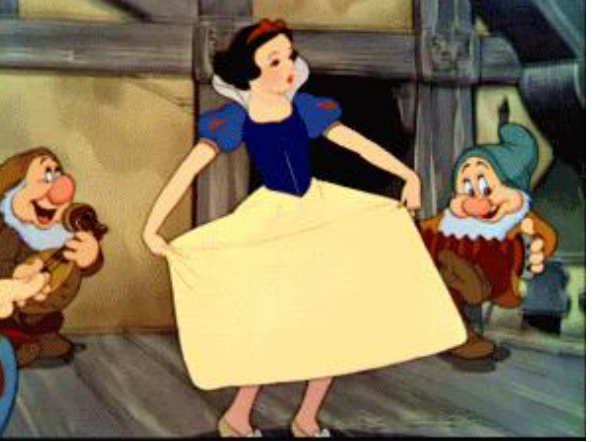
\includegraphics[width=65.52mm,height=121.47mm]{../../images/llm/page_031_img_01.png}%
\end{textblock*}

% deskripsi: Gambar stego-image yang terlihat identik dengan gambar cover, digunakan untuk menyembunyikan pesan.
% bbox normalisasi: [0.5430, 0.1230, 0.8550, 0.5320]
\begin{textblock*}{65.52mm}(114.03mm,36.53mm)
\noindent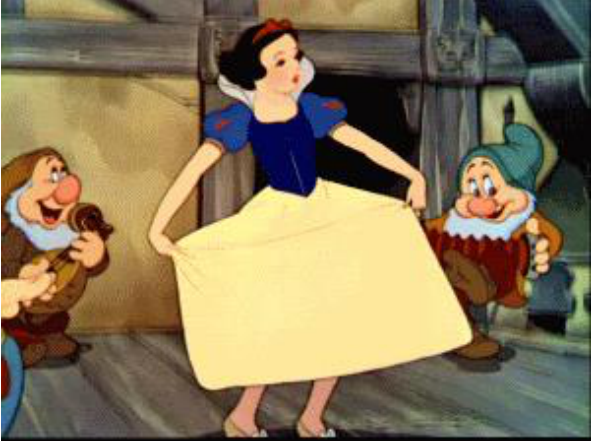
\includegraphics[width=65.52mm,height=121.47mm]{../../images/llm/page_031_img_02.png}%
\end{textblock*}

% deskripsi: Screenshot aplikasi Notepad yang berisi teks cerita Snow White sebagai pesan yang disembunyikan (embedded message).
% bbox normalisasi: [0.3770, 0.5960, 0.6650, 0.9070]
\begin{textblock*}{60.48mm}(79.17mm,177.01mm)
\noindent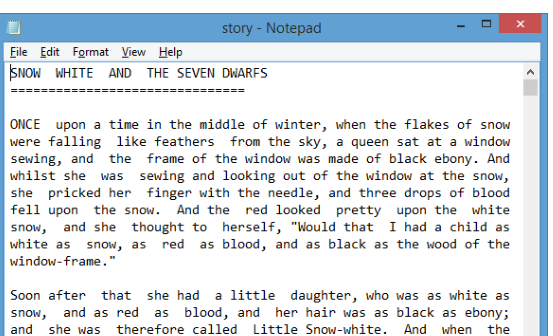
\includegraphics[width=60.48mm,height=92.37mm]{../../images/llm/page_031_img_03.png}%
\end{textblock*}

\end{document}
